\xchapter{Ambiente de trabalho e solução proposta}{}

Esta seção cobrirá as especificações do ambiente usado para realizar as medições. Veremos algumas soluções em tempo real para Linux e como elas funcionam. Também veremos os componentes da plataforma Raspberry e o módulo INTSight usado para realizar as medições.

\section{Soluções de SOTR Linux}

Existem várias maneiras de tornar o Linux um sistema operacional de tempo real, mas existem três maneiras principais de atingir esse objetivo. A primeira maneira é alterar a configuração do kernel durante a compilação, permitindo que as tarefas do kernel sejam interrompidas também. O segundo é organizar a ativação da tarefa a partir dos tipos de tratadores de interrupção. A terceira maneira é usar um nanokernel para intermediar o kernel com o hardware.

O patch Preempt-RT é o patch de tempo real padrão para o Raspberry e vários outros casos em que o Linux é usado. Torna o kernel completamente preemptivo para diminuir a latência de interrupção. O desenvolvimento é liderado por Ingo Molnar e tem a participação de muitos desenvolvedores em todo o mundo \cite{McKenney2005, Molnar2016}. Este trabalho analisou este patch.

Xenomai é um patch que usa a estratégia de nanokernel. Os nanokernels agem como uma camada extra de abstração entre o hardware e o kernel. Ele lida com interrupções de hardware e as define como interrupções para aplicativos em tempo real ou interrupções não críticas. Se for em tempo real, ele interrompe o kernel para que a tarefa seja executada imediatamente. Caso contrário, enfileire a tarefa para executar em outro momento \cite{Xenomai2005}.

\subsection{Preempt-RT}

As interrupções são capazes de interromper as tarefas que são executadas no espaço do usuário, mas às vezes as tarefas do kernel já levam um tempo considerável, portanto pode ser necessário interromper essas tarefas e dar lugar a uma tarefa de maior prioridade, como uma interrupção. Essa estratégia é chamada preempção. O kernel do Linux tem vários níveis de preempção:

\begin{itemize}
  \item PREEMPT\_NONE: as preempções ocorrem apenas nas tarefas do usuário.
  \item PREEMPT\_VOLUNTARY: algumas partes do kernel tem pontos específicos que permitem a preempção.
  \item CONFIG\_PREEMPT: semelhantes ao PREEMPT\_VOLUNTARY mas com uma região de preempção maior.
  \item PREEMPT\_RT\_FULL: praticamente qualquer seção do kernel pode ser preemptada, exceto algumas partes extremamente críticas.
\end{itemize}

\begin{figure}[!htb]
\centering
\subfloat[PREEMPT\_NONE]{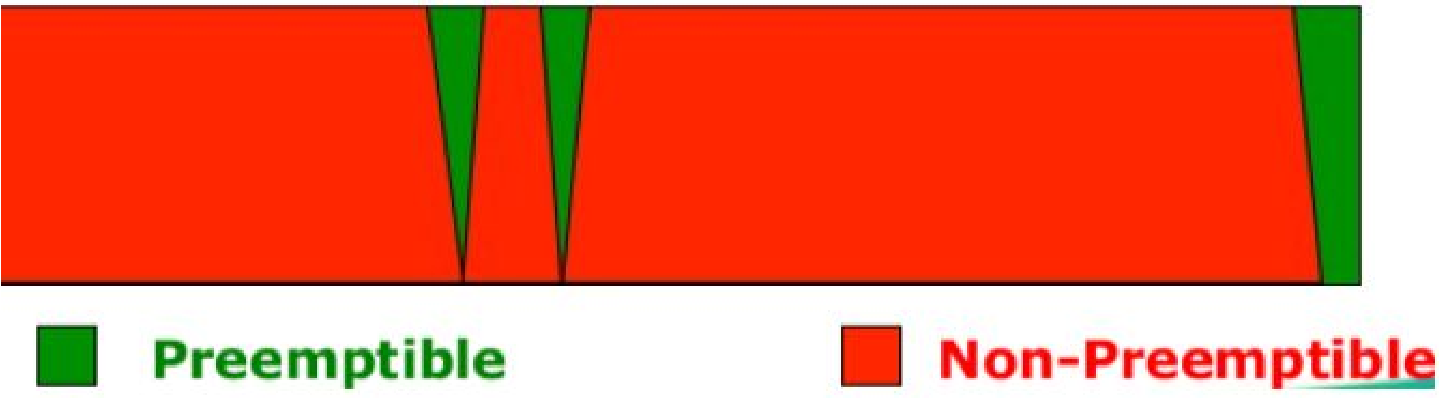
\includegraphics[width = .4\textwidth]{graficos/PREEMPT_NONE.png}}%
\subfloat[PREEMPT\_VOLUNTARY]{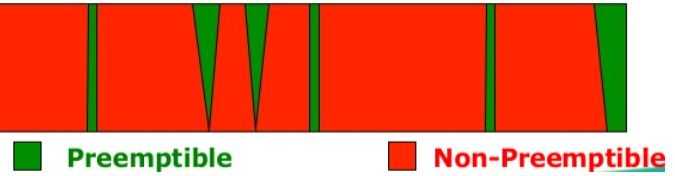
\includegraphics[width = .4\textwidth]{graficos/PREEMPT_VOLUNTARY.png}}\\
\subfloat[CONFIG\_PREEMPT]{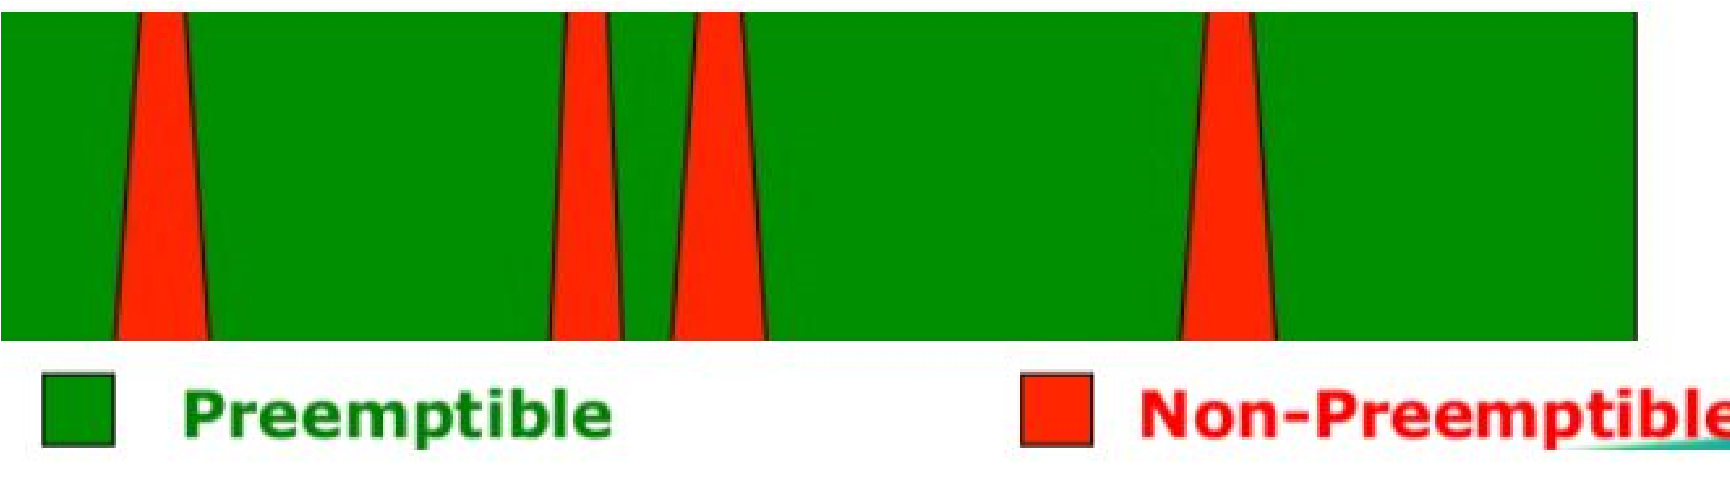
\includegraphics[width = .4\textwidth]{graficos/CONFIG_PREEMPT.png}}%
\subfloat[PREEMPT\_RT\_FULL]{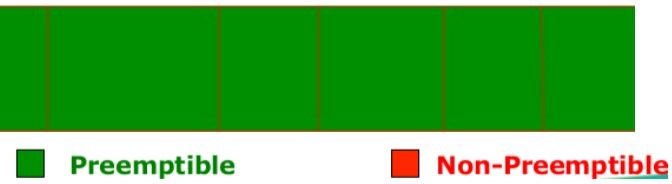
\includegraphics[width = .4\textwidth]{graficos/PREEMPT_RT_FULL.png}} 
\caption{Configurações de preempção no kernel \cite{Huang2017}}
\label{some example}
\end{figure}

Preempt-RT corresponde à configuração PREEMPT\_RT\_FULL. Nele, mesmo algumas seções críticas podem ser preemptadas, portanto, uma tarefa crítica pode acabar sendo movida para outro núcleo durante a execução. Quase todos os tratadores de interrupção são executados no contexto do processo no ambiente Preempt-RT, incluindo o Softirq, que será executado pela thread \textit{ksoftirqd}, permitindo que os tratadores sejam interrompidos. As exceções são a invocação do RCU (read-copy update) e os \textit{timers}, que continuam com o Softirq tradicional. Isso aumenta a capacidade de resposta do kernel, mas diminui sua quantidade de trabalho realizada por tempo.

\section{Raspberry}

Raspberry é um computador completo, do tamanho de um cartão de crédito, com todo o hardware em uma única placa. Tem um preço acessível e é amplamente utilizado para projetos que exigem um computador portátil. Mantido pela Raspberry Foundation \cite{RPF2019}, seu principal objetivo é promover a educação em informática. O primeiro modelo foi lançado em 2012 e se tornou um enorme sucesso.

O modelo usado neste trabalho é o Raspberry Pi 3 Model B. Este modelo possui uma CPU Broadcom BCM2837 com quatro núcleos, 1,2 GHz de frequência, arquitetura de 64 bits, 1 GB de RAM, acesso WIFI, Bluetooth, entrada Ethernet, 40 pinos de uso geral, 4 entradas USB, saídas de áudio e vídeo, saída HDMI e slot para cartão microSD.

O sistema operacional padrão é o Linux na distribuição Raspbian, uma distribuição baseada no Debian. Qualquer outra distribuição compatível com a arquitetura ARM pode ser usada e o fabricante fornece um utilitário para ajudar na escolha e gravação do sistema operacional em um cartão SD, que será a principal memória de dados do Raspberry.

\section{Módulos INTSpect e INTSight}

Em sistemas computacionais complexos, o número de variáveis é tão grande que não há um cálculo que possa ser feito para prever o tempo que uma interrupção leva para ser tratada, pois não basta levar em consideração a especificação de hardware, que geralmente não é aberta para impedir que os segredos industriais sejam expostos aos concorrentes, você também deve levar em consideração toda a estrutura de software do sistema operacional. Portanto, a realização de medições empíricas é a melhor maneira de avaliar a latência do sistema em sistemas reais. No entanto, fazer essas medições nem sempre é trivial.

Com o parágrafo anterior em mente, Luis Gerhorst \cite{Gerhorst2018} desenvolveu uma ferramenta para ajudar os desenvolvedores a fazer essas medições e analisar o tempo de resposta. Esta ferramenta foi dividida em 2 módulos: INTSight, que é um módulo do kernel responsável por fazer medições, e INTSpect, que é um módulo para acionar benchmarks no INTSight.

O INTSight é capaz de medir a latência de interrupção e latência de ativação, suporta vários métodos de medição, gera dados de formato simples a serem analisados posteriormente para medições sem comprometimento e tira fotos do sistema antes das baterias de medição para tornar os resultados facilmente reproduzíveis. Os locais no código onde o INTSight faz medições são definidos em tempo de compilação. Isso troca flexibilidade para maior precisão de medição.

O INTSight tem a função de realizar medições de latência de ativação para os vários mecanismos disponíveis no Linux com o mínimo de interferência possível. Na inicialização, o INTSight aloca uma rotina de serviço de interrupção (ISR) e um softirq, tasklet ou workqueue usado para o teste. Para considerar as variações que ocorrem, o número de medições pode ser definido. No início de cada medição, uma thread coordena a ativação da interrupção usando um mecanismo dependente da plataforma.

O método de medição utilizado foik\_time\_mono\_fast, porque é o segundo método de menor custo dentre os apresentados por Luis. O método com menor custo para uma plataforma ARM seria usar o PMCCNTR (Performance Monitors Cycle Count Register), que é um registrador específico que conta o número de pulsos de clock que ocorreram na CPU, portanto, lê-los tem o custo de leitura de um registrador. Na medição feita por ele, foi utilizada uma placa de núcleo único. Conhecendo a frequência de operação da CPU, é possível saber o tempo decorrido executando uma conta simples. No Raspberry, temos uma CPU de quatro núcleos e não temos garantia de que o núcleo que lidará com a interrupção seja o mesmo que o acionou. Como cada núcleo tem seu próprio contador, os valores não podem ser comparados. Para continuar com esse método de medição, você precisaria usar apenas um núcleo Raspberry, desativando os outros ou inserindo outro mecanismo de sincronização. Isso mudaria o comportamento real da CPU do Raspberry e resultaria em algo que não é comparável a uma situação de uso real.

Para gerar as interrupções de hardware no Raspberry, foram utilizados os pinos 16 e 18, BCM23 e BCM24, respectivamente. Um dos pinos estava no modo de escrita, enviando um sinal para o outro, definido no modo de leitura. O Raspberry usa 3,3 V em seus pinos digitais e o guia de uso indica que não deve ter uma corrente maior que 16 mA na entrada do pino, portanto, um resistor de 300 ohm foi usado para fazer a conexão entre os pinos.

\begin{figure}[!htb]
    \centering
    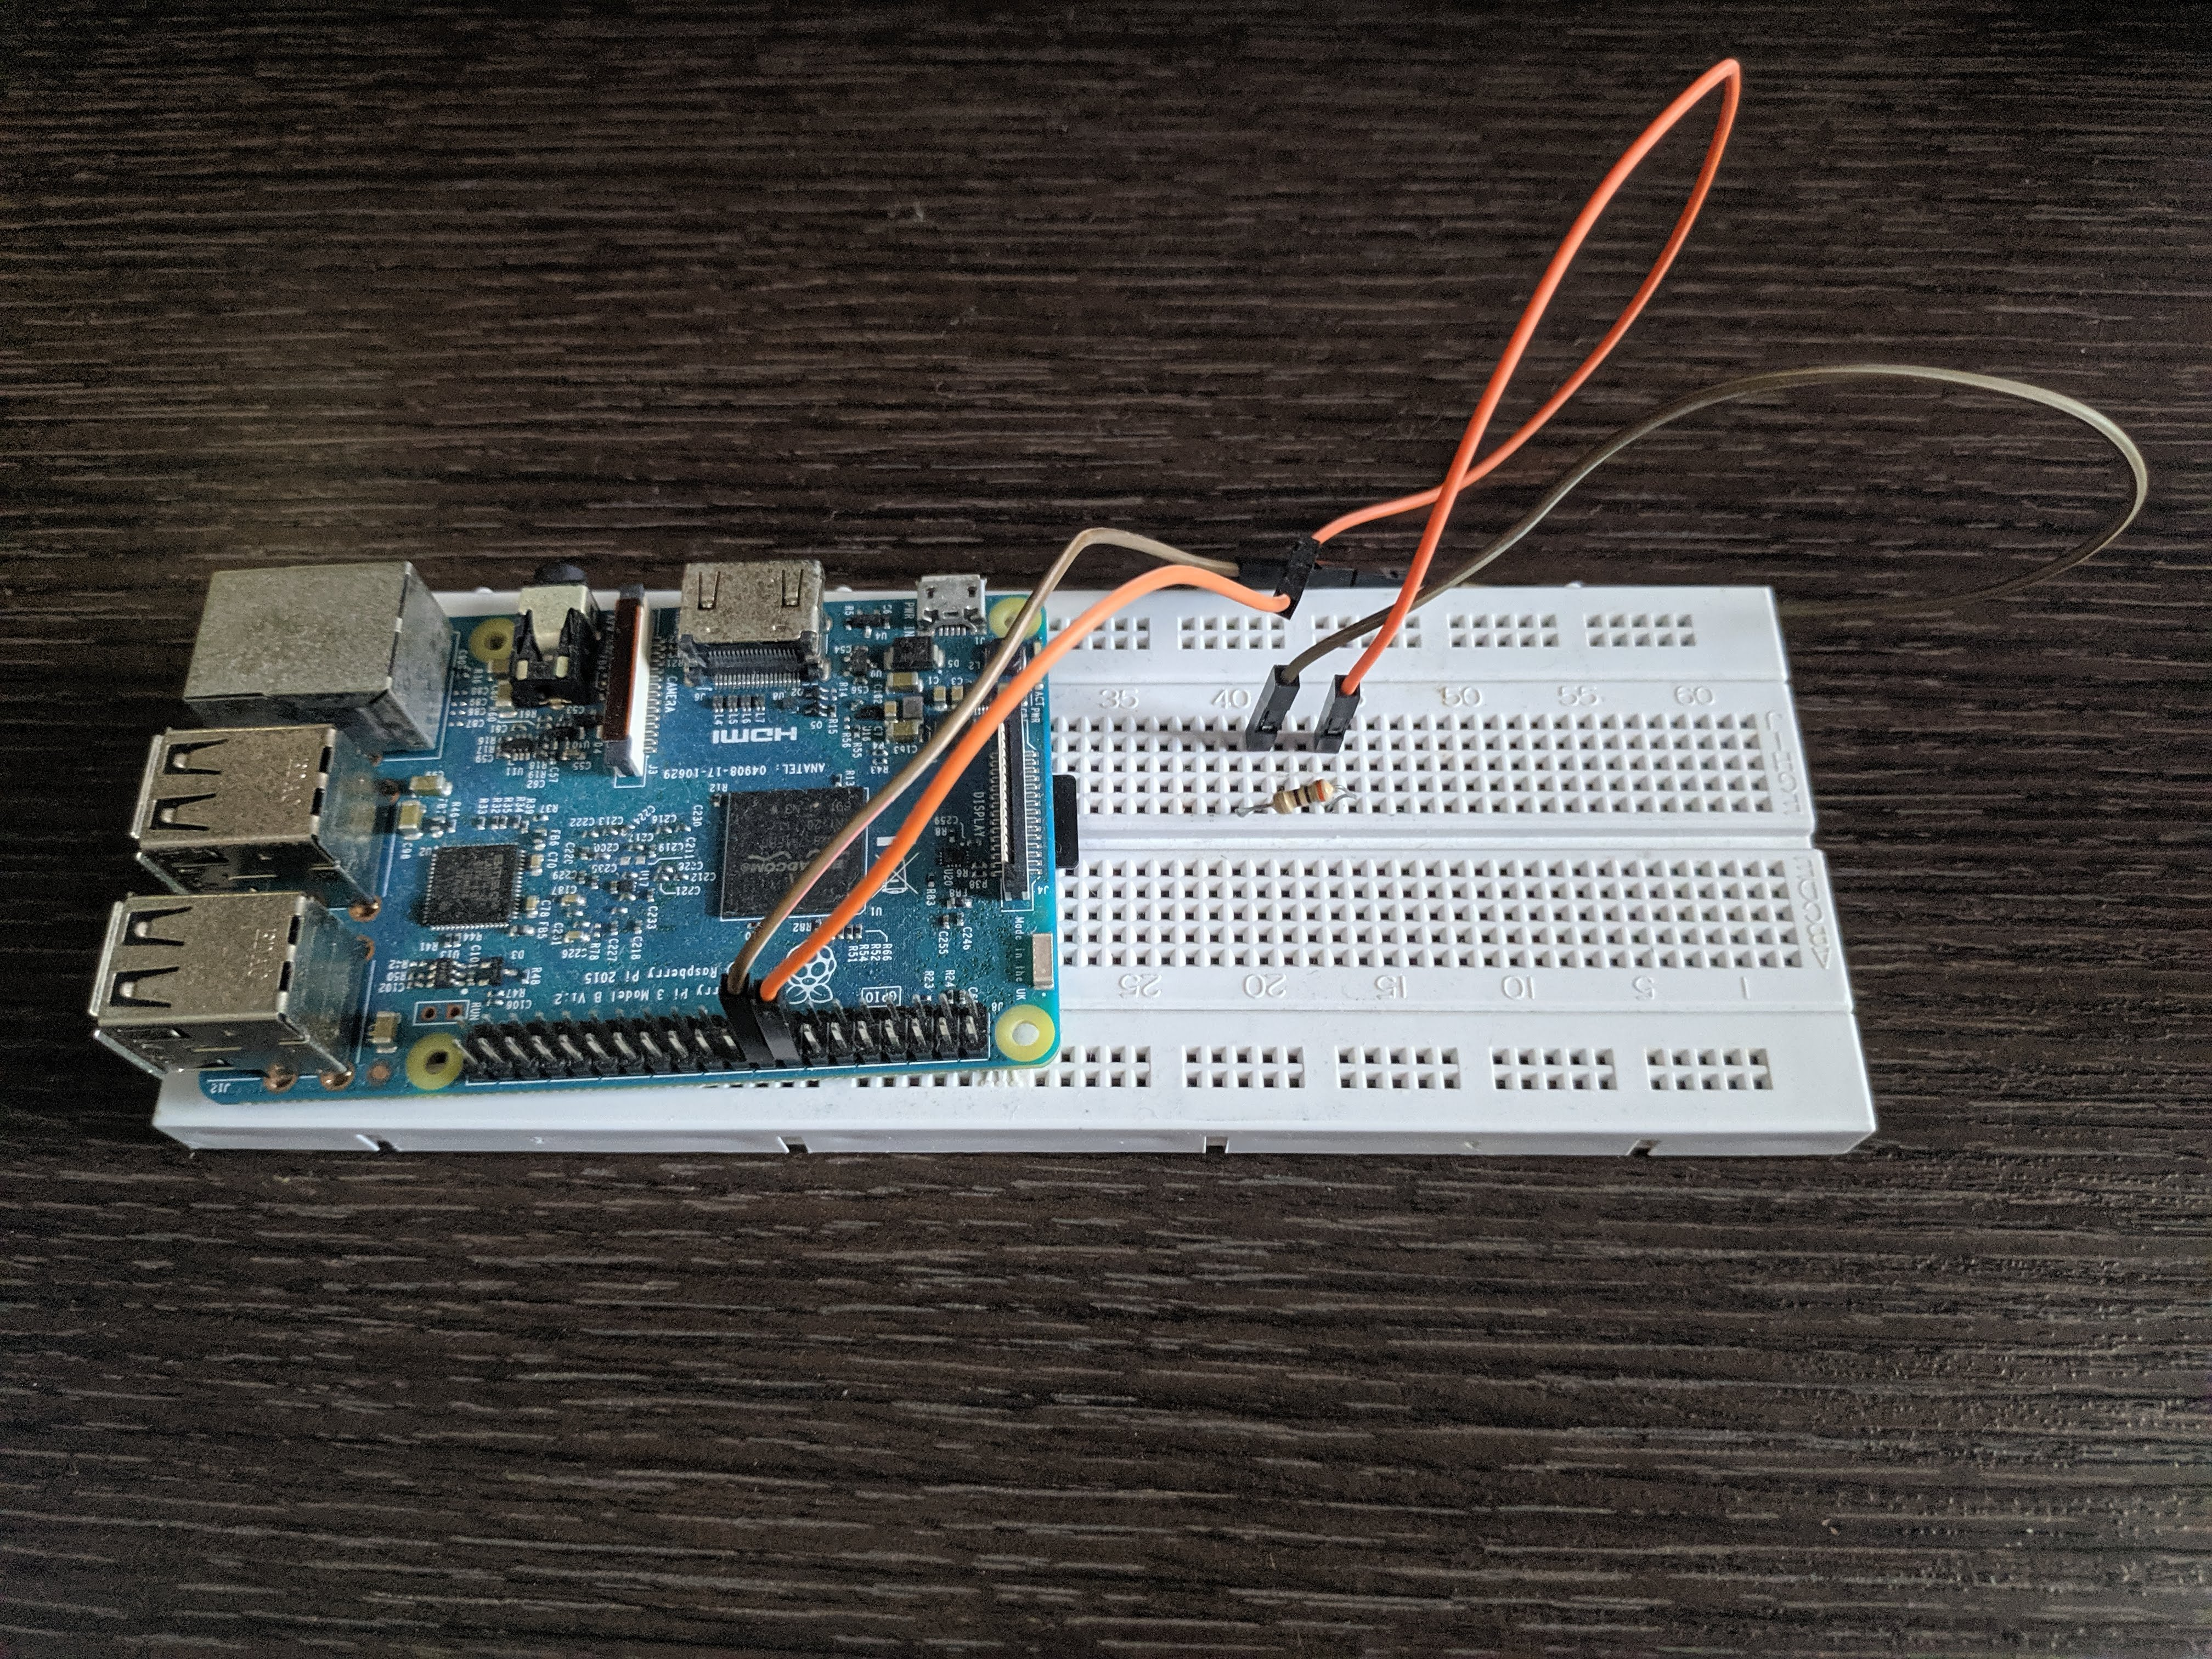
\includegraphics[width=.8\textwidth]{photos/raspberry-photo.jpg}
    \caption{Foto do Raspberry}
    \label{foto:raspberry}
\end{figure}
